Para probar que nuestro algoritmo no siempre da la solución óptima, vamos a presentar una familia que no solo nuestro algoritmo no encuentra la cota, sino también demostramos que no es \emph{k-acotado}, para ningún $k$ finito.

%TODO crear y agregar figura que represente la familia

$G_n$ de la familia \emph{3-caminos} para $n \geq 5$ esta compuesto por n nodos que se dividen en tres camino simples entre los nodos $1$ y $n$. A estos caminos los llamaremos $a$, $b$ y $c$ respectivamente. Los nodos se dividirán indiferentemente entre estos 3 caminos, pero cumpliendo que el costo total de cada camino sera:

$\bullet$ $w_1(a) = k+1$ \ $w_2(a)=1$

$\bullet$ $w_1(b) = k$  \ \ \ \ \ \ $w_2(b)=Q$

$\bullet$ $w_1(c) = 1$ \ \ \ \ \ \   $w_2(c)=i*Q$


\begin{figure}[H]
  \begin{center}
  \begin{minipage}{0.5\linewidth}
    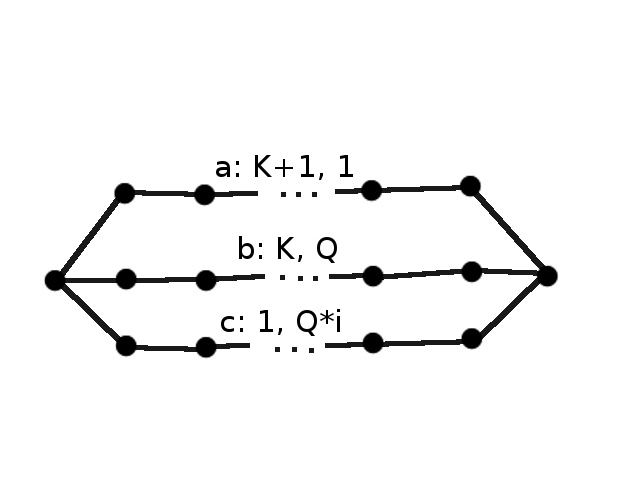
\includegraphics[width=\linewidth]{graficos/grafoFamiliaRompe.png}
    \caption{Familia \emph{3-caminos}}\label{fig:familia1}
  \end{minipage}
  \end{center}
\end{figure}

Con $k$ la cota sobre $w_1$, $i$ sera la proporción entre el resultado de nuestro algoritmo y el óptimo y $Q$ sera seleccionado para cumplir la condición anterior.

La idea de esta familia es que $a$ sea un camino donde se supera la cota por muy poco, pero tenga un $w_2$ muy bajo, $b$ sea el camino óptimo y su valor de $w_1$ sea exactamente $k$ y $c$ sea el camino que encuentra nuestro algoritmo, que tiene un $w_1$ muy bajo pero $w_2 = i * w_2(b)$.

Esto va a suceder ya que no va a existir ningún $p$ para el cual el camino $b$ sea mejor que los otros dos al mismo tiempo. Para $p$ muy chiquitos $b$ sera mejor que $a$ y para $p$ muy grandes sera mejor que $c$. Claramente si se cumple lo anterior no abra ningún $p$ que sea mejor que ambas.

\textbf{Demostración:}

Primero veamos como tiene que ser $p$ para que $b$ sea menor que $a$.

Sea $p$ tal que 

$(1-p)*w_1(b)+p*w_2(b) < (1-p)*w_1(a)+p*w_2(a)$

$(1-p)*k+p*Q < (1-p)*(k+1)+p$

$k-p*k+p*Q < k-p*k-p+1+p$

$p*Q < 1$

$p < \frac{1}{Q}$ Para que $b$ sea mejor que $a$

Ahora veamos como tiene que ser $p$ para que $b$ sea menor que $c$.

Sea $p$ tal que 

$(1-p)*w_1(b)+p*w_2(b) < (1-p)*w_1(c)+p*w_2(c)$

$(1-p)*k+p*Q < (1-p)+p*i*Q$

$k-p*k+p*Q < 1-p+p*i*Q$

$k-1 < -p+p*i*Q+p*k-p*Q$

$k-1 < p*(-1+i*Q+k-Q)$

$\frac{k-1}{-1+i*Q+k-Q} < p$ Tomando $k,i > 1$, ya que $k > 1$ y $Q*i > Q \rightarrow i*Q-Q+k-1 > 0$ por $Q > 0$

Para que $b$ sea mejor que $a$ y $c$ se debería cumplir:

$\frac{k-1}{-1+i*Q+k-Q} < p < \frac{1}{Q}$

Para forzar que esto no ocurra buscamos $k$ y $Q$ tal que:

$\frac{k-1}{i*Q-Q+k-1} > \frac{1}{Q}$

$k-1 > \frac{i*Q-Q+k-1}{Q}$ ya que $i*Q-Q+k-1 > 0$ como vimos en el punto anterior

$k-1 > \frac{k-1}{Q}+i-1$

$(k-1) \frac{Q-1}{Q} > i-1$

Tomando $Q=3$ y $k=2*i-1$

$(2*i-2) \frac{2}{3} > i-1$

$(i-1) \frac{4}{3} > i-1$

$(i-1) \frac{1}{3} > 0$

$i-1 > 0$

$i > 1$ Como ya habíamos dicho antes.


O sea la familia para un $n$ y un $i$ dado estaría conformada por:

$k = 2*i-1$

$\bullet$ $w_1(a) = 2*i$, $w_2(a)=1$

$\bullet$ $w_1(b) = 2*i-1$, $w_2(b)=3$

$\bullet$ $w_1(c) = 1$, $w_2(c)=i*3$

Veamos que para cualquier $i$, la proporción entre el camino encontrado en la golosa y el exacto es $i$:

Como demostramos previamente nuestro algoritmo va a encontrar el camino $c$ que tiene $w_2=i*3$, y el camino óptimo es el $b$, con $w_2=3$. Por los que claramente la proporción es $i$, $\frac{3i}{3}=i$.

Para armar un grafo de esta familia hay diversas formas.Siempre se fijan 2 nodos como el inicial y el final. Los demás nodos se distribuyen entre tres caminos disjuntos en nodos, de forma arbitraria. Particularmente nuestra implementación distribuimos equitativamente los nodos entre los 3 caminos. (Los nodos sobrantes , $(n-2) mod 3$, los dejamos como nodos aislados por un tema de facilidad).

Luego queda asignar los pesos a las aristas, hay que distribuir el peso de cada camino entre las aristas del mismo. Otra vez esto puede hacerse arbitrariamente, y en nuestro caso buscamos una distribución uniforme.
En el caso de pesos reales, se divide el peso total del camino por la cantidad de aristas y se asigna ese peso a cada arista.
En el caso de pesos enteros esto no se puede realizar porque no podemos asegurar que sea divisible. Para asegurarnos multiplicamos los pesos de los 3 caminos por la cantidad de aristas de un camino (las 3 tienen la misma cantidad) para asegurarnos que sea divisible. Esto no afecta nada del análisis anterior ya que al multiplicar a todos los caminos por un mismo número no afecta ni la elección del algoritmo ni la proporción.

Cabe aclarar que esta familia se puede extender agregando cualquier cantidad de nodos y aristas arbitrarias, siempre y cuando el camino $b$ siga siendo el único óptimo. En esta extensión el goloso nunca encontrará el óptimo ya que al agregar otras opciones no afecta que no exista ningún $p$ para el cual el camino $b$ (óptimo) sea mejor que todos los demás, ya que no puede ser mejor que $a$ y $c$ al mismo tiempo. Pero al extender la familia lo que si se pierde es el análisis de	qué tan mala puede ser la solución.  